% LyX 2.2.2 created this file.  For more info, see http://www.lyx.org/.
%% Do not edit unless you really know what you are doing.
\documentclass[ruled]{article}
\usepackage{courier}
\usepackage[T1]{fontenc}
\usepackage[latin9]{inputenc}
\usepackage[letterpaper]{geometry}
\geometry{verbose}
\usepackage{color}
\usepackage{url}
\usepackage{algorithm2e}
\usepackage{amsmath}
\usepackage{amssymb}
\usepackage[unicode=true,
 bookmarks=false,
 breaklinks=false,pdfborder={0 0 1},backref=section,colorlinks=true]
 {hyperref}

\usepackage{color}
\usepackage{minted}
\usepackage{graphicx}
\newminted[python]{python}{frame=single}
\fvset{showspaces}
\renewcommand\FancyVerbSpace{\textcolor{white}{\char32}}
\makeatletter


%%%%%%%%%%%%%%%%%%%%%%%%%%%%%% LyX specific LaTeX commands.
\providecommand{\LyX}{\texorpdfstring%
  {L\kern-.1667em\lower.25em\hbox{Y}\kern-.125emX\@}
  {LyX}}
%% Special footnote code from the package 'stblftnt.sty'
%% Author: Robin Fairbairns -- Last revised Dec 13 1996
\let\SF@@footnote\footnote
\def\footnote{\ifx\protect\@typeset@protect
    \expandafter\SF@@footnote
  \else
    \expandafter\SF@gobble@opt
  \fi
}
\expandafter\def\csname SF@gobble@opt \endcsname{\@ifnextchar[%]
  \SF@gobble@twobracket
  \@gobble
}
\edef\SF@gobble@opt{\noexpand\protect
  \expandafter\noexpand\csname SF@gobble@opt \endcsname}
\def\SF@gobble@twobracket[#1]#2{}

%%%%%%%%%%%%%%%%%%%%%%%%%%%%%% Textclass specific LaTeX commands.
\newenvironment{lyxcode}
{\par\begin{list}{}{
\setlength{\rightmargin}{\leftmargin}
\setlength{\listparindent}{0pt}% needed for AMS classes
\raggedright
\setlength{\itemsep}{0pt}
\setlength{\parsep}{0pt}
\normalfont\ttfamily}%
 \item[]}
{\end{list}}

\@ifundefined{date}{}{\date{}}
%%%%%%%%%%%%%%%%%%%%%%%%%%%%%% User specified LaTeX commands.
\definecolor{mygreen}{rgb}{0,0.6,0}
\definecolor{mygray}{rgb}{0.5,0.5,0.5}
\definecolor{mymauve}{rgb}{0.58,0,0.82}

\makeatother

\usepackage{listings}
\lstset{backgroundcolor={\color{white}},
basicstyle={\footnotesize\ttfamily},
breakatwhitespace=false,
breaklines=true,
captionpos=b,
commentstyle={\color{mygreen}},
deletekeywords={...},
escapeinside={\%*}{*)},
extendedchars=true,
frame=shadowbox,
keepspaces=true,
keywordstyle={\color{blue}},
language=Python,
morekeywords={*,...},
numbers=none,
numbersep=5pt,
numberstyle={\tiny\color{mygray}},
rulecolor={\color{black}},
showspaces=false,
showstringspaces=false,
showtabs=false,
stepnumber=1,
stringstyle={\color{mymauve}},
tabsize=2}
\begin{document}
\global\long\def\reals{\mathbf{R}}
 \global\long\def\integers{\mathbf{Z}}
\global\long\def\naturals{\mathbf{N}}
 \global\long\def\rationals{\mathbf{Q}}
\global\long\def\ca{\mathcal{A}}
\global\long\def\cb{\mathcal{B}}
 \global\long\def\cc{\mathcal{C}}
 \global\long\def\cd{\mathcal{D}}
\global\long\def\ce{\mathcal{E}}
\global\long\def\cf{\mathcal{F}}
\global\long\def\cg{\mathcal{G}}
\global\long\def\ch{\mathcal{H}}
\global\long\def\ci{\mathcal{I}}
\global\long\def\cj{\mathcal{J}}
\global\long\def\ck{\mathcal{K}}
\global\long\def\cl{\mathcal{L}}
\global\long\def\cm{\mathcal{M}}
\global\long\def\cn{\mathcal{N}}
\global\long\def\co{\mathcal{O}}
\global\long\def\cp{\mathcal{P}}
\global\long\def\cq{\mathcal{Q}}
\global\long\def\calr{\mathcal{R}}
\global\long\def\cs{\mathcal{S}}
\global\long\def\ct{\mathcal{T}}
\global\long\def\cu{\mathcal{U}}
\global\long\def\cv{\mathcal{V}}
\global\long\def\cw{\mathcal{W}}
\global\long\def\cx{\mathcal{X}}
\global\long\def\cy{\mathcal{Y}}
\global\long\def\cz{\mathcal{Z}}
\global\long\def\ind#1{1(#1)}
\global\long\def\pr{\mathbb{P}}

\global\long\def\ex{\mathbb{E}}
\global\long\def\var{\textrm{Var}}
\global\long\def\cov{\textrm{Cov}}
\global\long\def\sgn{\textrm{sgn}}
\global\long\def\sign{\textrm{sign}}
\global\long\def\kl{\textrm{KL}}
\global\long\def\law{\mathcal{L}}
\global\long\def\eps{\varepsilon}
\global\long\def\convd{\stackrel{d}{\to}}
\global\long\def\eqd{\stackrel{d}{=}}
\global\long\def\del{\nabla}
\global\long\def\loss{\ell}
\global\long\def\tr{\operatorname{tr}}
\global\long\def\trace{\operatorname{trace}}
\global\long\def\diag{\text{diag}}
\global\long\def\rank{\text{rank}}
\global\long\def\linspan{\text{span}}
\global\long\def\proj{\text{Proj}}
\global\long\def\argmax{\operatornamewithlimits{arg\, max}}
\global\long\def\argmin{\operatornamewithlimits{arg\, min}}
\global\long\def\bfx{\mathbf{x}}
\global\long\def\bfy{\mathbf{y}}
\global\long\def\bfl{\mathbf{\lambda}}
\global\long\def\bfm{\mathbf{\mu}}
\global\long\def\calL{\mathcal{L}}
\global\long\def\vw{\boldsymbol{w}}
\global\long\def\vx{\boldsymbol{x}}
\global\long\def\vxi{\boldsymbol{\xi}}
\global\long\def\valpha{\boldsymbol{\alpha}}
\global\long\def\vbeta{\boldsymbol{\beta}}
\global\long\def\vsigma{\boldsymbol{\sigma}}
\global\long\def\vmu{\boldsymbol{\mu}}
\global\long\def\vtheta{\boldsymbol{\theta}}
\global\long\def\vd{\boldsymbol{d}}
\global\long\def\vs{\boldsymbol{s}}
\global\long\def\vt{\boldsymbol{t}}
\global\long\def\vh{\boldsymbol{h}}
\global\long\def\ve{\boldsymbol{e}}
\global\long\def\vf{\boldsymbol{f}}
\global\long\def\vg{\boldsymbol{g}}
\global\long\def\vz{\boldsymbol{z}}
\global\long\def\vk{\boldsymbol{k}}
\global\long\def\va{\boldsymbol{a}}
\global\long\def\vb{\boldsymbol{b}}
\global\long\def\vv{\boldsymbol{v}}
\global\long\def\vy{\boldsymbol{y}}


\title{Machine Learning and Computational Statistics\\
Homework 6: Ensemble Methods}
\author{Zhuoru Lin}
\maketitle
\textbf{Due: TBD in week after test, at 10pm (Submit via Gradescope)}

\textbf{Instructions}: Your answers to the questions below, including
plots and mathematical work, should be submitted as a single PDF file.
It's preferred that you write your answers using software that typesets
mathematics (e.g. \LaTeX{}, \LyX{}, or MathJax via iPython), though
if you need to you may scan handwritten work. You may find the \href{https://github.com/gpoore/minted}{minted}
package convenient for including source code in your \LaTeX{} document.
If you are using \LyX{}, then the \href{https://en.wikibooks.org/wiki/LaTeX/Source_Code_Listings}{listings}
package tends to work better.

%%%%%%%%%%%%%%%%%%%%%%%%%%%%%%%%%%%%%%%%%%%%%%%%%%%%%%%%%%%%%%%%
%1 Gradient Boosting Machine
%%%%%%%%%%%%%%%%%%%%%%%%%%%%%%%%%%%%%%%%%%%%%%%%%%%%%%%%%%%%%%%%
\section{Gradient Boosting Machines}

Recall the general gradient boosting algorithm\footnote{Besides the lecture slides, you can find an accessible discussion
of this approach in \url{http://www.saedsayad.com/docs/gbm2.pdf},
in one of the original references \url{http://statweb.stanford.edu/~jhf/ftp/trebst.pdf},
and in this review paper \url{http://web.stanford.edu/~hastie/Papers/buehlmann.pdf}. }, for a given loss function $\ell$ and a hypothesis space $\cf$
of regression functions (i.e. functions mapping from the input space
to $\reals$): 
\begin{enumerate}
\item Initialize $f_{0}(x)=0$. 
\item For $m=1$ to $M$:

\begin{enumerate}
\item Compute: 
\[
{\bf g}_{m}=\left(\left.\frac{\partial}{\partial f(x_{j})}\sum_{i=1}^{n}\ell\left(y_{i},f(x_{i})\right)\right|_{f(x_{i})=f_{m-1}(x_{i}),\,i=1,\ldots,n}\right)_{j=1}^{n}
\]
\item Fit regression model to $-{\bf g}_{m}$: 
\[
h_{m}=\argmin_{h\in\cf}\sum_{i=1}^{n}\left(\left(-{\bf g}_{m}\right)_{i}-h(x_{i})\right)^{2}.
\]
\item Choose fixed step size $\nu_{m}=\nu\in(0,1]$, or take 
\[
\nu_{m}=\argmin_{\nu>0}\sum_{i=1}^{n}\ell\left(y_{i},f_{m-1}(x_{i})+\nu h_{m}(x_{i})\right).
\]
\item Take the step: 
\[
f_{m}(x)=f_{m-1}(x)+\nu_{m}h_{m}(x)
\]
\end{enumerate}
\item Return $f_{M}$. 
\end{enumerate}
In this problem we'll derive two special cases of the general gradient
boosting framework: $L_{2}$-Boosting and BinomialBoost. 


\begin{enumerate}
%%%%%%%%%%%%%%%%%%%%%%%%%%%%%%%%%%%%%%%%%%%%%%%%%%%%%%%%%%%%%%%%
%1.1 
%%%%%%%%%%%%%%%%%%%%%%%%%%%%%%%%%%%%%%%%%%%%%%%%%%%%%%%%%%%%%%%%
\item Consider the regression framework, where $\cy=\reals$. Suppose our
loss function is given by 
\[
\ell(\hat{y},y)=\frac{1}{2}\left(\hat{y}-y\right)^{2},
\]
and at the beginning of the $m$'th round of gradient boosting, we
have the function $f_{m-1}(x)$. Show that the $h_{m}$ chosen as
the next basis function is given by 
\[
h_{m}=\argmin_{h\in\cf}\sum_{i=1}^{n}\left[\left(y_{i}-f_{m-1}(x_{i})\right)-h(x_{i})\right]^{2}.
\]
In other words, at each stage we find the weak prediction function
$h_{m}\in\cf$ that is the best fit to the residuals from the previous
stage. {[}Hint: Once you understand what's going on, this is a pretty
easy problem.{]} 
%%%%%%%%%%%%%%%%%%%%%%%%%%%%%%%%%%%%%%%%%%%%%%%%%%%%%%%%%%%%%%%%
% 1.1 Answer
%%%%%%%%%%%%%%%%%%%%%%%%%%%%%%%%%%%%%%%%%%%%%%%%%%%%%%%%%%%%%%%%
\\
\noindent\rule{14.3cm}{2pt}
\textbf{Answer:}\\
The negative gradient direction of $\ell$ can be calculated by:
\[
-\frac{\partial \ell(\hat{y},y)}{\partial \hat{y}} = -(\hat{y}-y) = y-\hat{y}=y-f(x)
\]
$h_m$ is chosen to minimize the square error with $-\frac{\partial \ell(\hat{y},y)}{\partial \hat{y}}$, therefore:
\[
h_{m}=\argmin_{h\in\cf}\sum_{i=1}^{n}\left[\left(y_{i}-f_{m-1}(x_{i})\right)-h(x_{i})\right]^{2}.
\]
%%%%%%%%%%%%%%%%%%%%%%%%%%%%%%%%%%%%%%%%%%%%%%%%%%%%%%%%%%%%%%%%
% 1.2
%%%%%%%%%%%%%%%%%%%%%%%%%%%%%%%%%%%%%%%%%%%%%%%%%%%%%%%%%%%%%%%%
\pagebreak
\item Now let's consider the classification framework, where $\cy=\left\{ -1,1\right\} $.
In lecture, we noted that AdaBoost corresponds to forward stagewise
additive modeling with the exponential loss, and that the exponential
loss is not very robust to outliers (i.e. outliers can have a large
effect on the final prediction function). Instead, let's consider
the logistic loss 
\[
\ell(m)=\ln\left(1+e^{-m}\right),
\]
where $m=yf(x)$ is the margin. Similar to what we did in the $L_{2}$-Boosting
question, write an expression for $h_{m}$ as an argmin over $\cf$.
%%%%%%%%%%%%%%%%%%%%%%%%%%%%%%%%%%%%%%%%%%%%%%%%%%%%%%%%%%%%%%%%
% 1.2 Answer
%%%%%%%%%%%%%%%%%%%%%%%%%%%%%%%%%%%%%%%%%%%%%%%%%%%%%%%%%%%%%%%%
\\
\noindent\rule{14.3cm}{2pt}\\
\textbf{Answer:}
The negative gradient direction is calculated by:
\[
-\frac{\partial \ell(y,f(x))}{\partial f(x)}=\frac{ye^{-yf(x)}}{1+e^{-yf(x)}}
\]
$h_m$ is chosen by:
\[
\argmin_{h \in \cf} \sum_{i=1}^{n}\left[ \frac{y_{i}e^{-y_{i}f(x_{i})}}{1+e^{-y_{i}f(x_{i})}}-h(x_i)  \right]^2
\]
\end{enumerate}

\pagebreak
\section{From Margins to Conditional Probabilities\protect\footnote{This problem is based on Section 7.5.3 of Schapire and Freund's book
\emph{Boosting: Foundations and Algorithms}.}}

Let's consider the classification setting, in which $\left(x_{1},y_{1}\right),\ldots,\left(x_{n},y_{n}\right)\in\cx\times\left\{ -1,1\right\} $
are sampled i.i.d. from some unknown distribution. For a prediction
function $f:\cx\to\reals$, we define the \textbf{margin }on an example
$\left(x,y\right)$ to be $m=yf(x)$. Since our class predictions
are given by $\sign(f(x))$, we see that a prediction is correct iff
$m(x)>0$. We have said we can interpret the magnitude of the margin
$\left|m(x)\right|$ as a measure of confidence. However, it is not
clear what the ``units'' of the margin are, so it is hard to interpret
the magnitudes beyond saying one prediction is more or less confident
than another. In this problem, we investigate how we can translate
the margin into a conditional probability, which is much easier to
interpret. In other words, we are looking for a mapping $m(x)\mapsto p(y=1\mid x)$. 

In this problem we will consider margin-based losses. A loss function
is a \textbf{margin-based loss }if it can be written in terms of the
margin $m=yf(x)$. We are interested in how we can go from an empirical
risk minimizer of a margin loss, $\hat{f}=\argmin_{f\in\cf}\sum_{i=1}^{n}\ell\left(y_{i}f(x_{i})\right)$,
to a conditional probability estimator $\hat{\pi}(x)\approx p(y=1\mid x)$.
Our approach will be to try to find a way to use the Bayes prediction
function\footnote{In this context, the Bayes prediction function is often referred to
as the ``population minimizer.'' In our case, ``population'' referes
to the fact that we are minimizing with respect to the true distribution,
rather than a sample. The term ``population'' arises from the context
where we are using a sample to approximate some statistic of an entire
population (e.g. a population of people or trees).} $f^{*}=\argmin_{f}\ex_{x,y}\left[\ell(yf(x)\right]$ to get the true
conditional probability $p(y=1\mid x$), and then apply the same mapping
to the empirical risk minimizer. While there is plenty that can go
wrong with this ``plug-in'' approach (primarily, the empirical risk
minimizer from a hypothesis space $\cf$ may be a poor estimate for
the Bayes prediction function), it is at least well-motivated, and
it can work well in practice. And \textbf{please note} that we can
do better than just hoping for success: if you have enough validation
data, you can directly assess how well ``calibrated'' the predicted
probabilities are. This blog post has some discussion of calibration
plots: \href{https://jmetzen.github.io/2015-04-14/calibration.html}{https://jmetzen.github.io/2015-04-14/calibration.html}. 

It turns out it is straightforward to find the Bayes prediction function
$f^{*}$ for margin losses, at least in terms of the data-generating
distribution: For any given $x\in\cx$, we'll find the best possible
prediction $\hat{y}$. This will be the $\hat{y}$ that minimizes
\[
\ex_{y}\left[\ell\left(y\hat{y}\right)\mid x\right].
\]
If we can calculate this $\hat{y}$ for all $x\in\cx$, then we will
have determined $f^{*}(x)$. We will simply take
\[
f^{*}(x)=\argmin_{\hat{y}}\ex_{y}\left[\ell\left(y\hat{y}\right)\mid x\right].
\]

Below we'll calculate $f^{*}$ for several loss functions. It will
be convenient to let $\pi(x)=\pr\left(y=1\mid x\right)$ in the work
below.
\begin{enumerate}
%%%%%%%%%%%%%%%%%%%%%%%%%%%%%%%%%%%%%%%%%%%%%%%%%%%%%%%%%%%%%%%%
% 2.1 
%%%%%%%%%%%%%%%%%%%%%%%%%%%%%%%%%%%%%%%%%%%%%%%%%%%%%%%%%%%%%%%%
\item Write $\ex_{y}\left[\ell\left(yf(x)\right)\mid x\right]$ in terms
of $\pi(x)$ and $\ell\left(f(x)\right)$. {[}Hint: Use the fact that
$y\in\left\{ -1,1\right\} $.{]}
%%%%%%%%%%%%%%%%%%%%%%%%%%%%%%%%%%%%%%%%%%%%%%%%%%%%%%%%%%%%%%%%
% 2.1 Answer
%%%%%%%%%%%%%%%%%%%%%%%%%%%%%%%%%%%%%%%%%%%%%%%%%%%%%%%%%%%%%%%%
\\
\noindent\rule{14.5cm}{2pt}\\
\textbf{Answer:}\\
\[
\pi(x)\ell(f(x))+(1-\pi(x)\ell(-f(x))
\]
\pagebreak
%%%%%%%%%%%%%%%%%%%%%%%%%%%%%%%%%%%%%%%%%%%%%%%%%%%%%%%%%%%%%%%%
% 2.2
%%%%%%%%%%%%%%%%%%%%%%%%%%%%%%%%%%%%%%%%%%%%%%%%%%%%%%%%%%%%%%%%
\item Show that the Bayes prediction function $f^{*}(x)$ for the exponential
loss function $\ell\left(y,f(x)\right)=e^{-yf(x)}$ is given by 
\[
f^{*}(x)=\frac{1}{2}\ln\left(\frac{\pi(x)}{1-\pi(x)}\right)
\]
and, given the Bayes prediction function $f^{*}$, we can recover
the conditional probabilities by
\[
\pi(x)=\frac{1}{1+e^{-2f^{*}(x)}}.
\]
{[}Hint: Differentiate the expression in the previous problem with
respect to $f(x)$. To make things a little less confusing, and also
to write less, you may find it useful to change variables a bit: Fix
an $x\in\cx$. Then write $p=\pi(x)$ and $\hat{y}=f(x)$. After substituting
these into the expression you had for the previous problem, you'll
want to find $\hat{y}$ that minimizes the expression. Use differential
calculus. Once you've done it for a single $x$, it's easy to write
the solution as a function of $x$.{]} 
%%%%%%%%%%%%%%%%%%%%%%%%%%%%%%%%%%%%%%%%%%%%%%%%%%%%%%%%%%%%%%%%
% 2.2 Answer
%%%%%%%%%%%%%%%%%%%%%%%%%%%%%%%%%%%%%%%%%%%%%%%%%%%%%%%%%%%%%%%%
\\
\noindent\rule{14.3cm}{2pt}\\
\textbf{Answer:}\\
Let $R$ be the Bayes risk:
\begin{align}
	R = \ex_{y}\left[\ell\left(yf(x)\right)\mid x\right]&=\pi(x)e^{-f(x)}+(1-\pi(x))e^{f(x)} \nonumber\\
	\frac{\partial R}{f(x)}&=-\pi(x)e^{-f(x)}+(1+\pi(x))e^{f(x)}
\end{align}
The Bayes risk minimizer should have $\frac{\partial R}{f(x)}=0$.
\begin{align}
	\frac{\partial R}{f(x)}=0 \iff (1+\pi(x))e^{f^{*}(x)} &= \pi(x)e^{-f^{*}(x)} \nonumber\\
	\frac{e^{f^{*}(x)}}{e^{-f^{*}(x)}} &= \frac{\pi(x)}{1+\pi(x)} \nonumber	\\
	f^{*}(x) &= \frac{1}{2}(\frac{\pi(x)}{1-\pi(x)}) 
\end{align}

Rearrange (1) we get:
\begin{align*}
\pi(x)=\frac{1}{1+e^{-2f^{*}(x)}}.
\end{align*}

%%%%%%%%%%%%%%%%%%%%%%%%%%%%%%%%%%%%%%%%%%%%%%%%%%%%%%%%%%%%%%%%
% 2.3 
%%%%%%%%%%%%%%%%%%%%%%%%%%%%%%%%%%%%%%%%%%%%%%%%%%%%%%%%%%%%%%%%
\pagebreak
\item Show that the Bayes prediction function $f^{*}(x)$ for the logistic
loss function $\ell\left(y,f(x)\right)=\ln\left(1+e^{-yf(x)}\right)$
is given by
\[
f^{*}(x)=\ln\left(\frac{\pi(x)}{1-\pi(x)}\right)
\]
and the conditional probabilities are given by
\[
\pi(x)=\frac{1}{1+e^{-f^{*}(x)}}.
\]
 Again, we may assume that $\pi(x)\in(0,1)$.
%%%%%%%%%%%%%%%%%%%%%%%%%%%%%%%%%%%%%%%%%%%%%%%%%%%%%%%%%%%%%%%%
% 2.3 Answer
%%%%%%%%%%%%%%%%%%%%%%%%%%%%%%%%%%%%%%%%%%%%%%%%%%%%%%%%%%%%%%%%
\\
\noindent\rule{14.3cm}{2pt}\\
\textbf{Answer:}\\
Let $R$ be the Bayes risk:
\begin{align*}
R = \ex_{y}\left[\ell\left(yf(x)\right)\mid x\right]&=\pi(x)\ln(1+e^{-f(x)})+(1-\pi(x))\ln(1+e^{f(x)}) \nonumber\\
\end{align*}

\begin{align}
\frac{\partial R}{f(x)}=0 \implies (1-\pi(x))\frac{e^{f^{*}(x)}}{1+e^{f^{*}(x)}}&=\pi(x)\frac{e^{-f^{*}(x)}}{1+e^{-f^{*}(x)}}\\
e^{f*(x)}&=\frac{\pi(x)}{1-\pi(x)}\\
f^{*}(x) &= \ln \frac{\pi(x)}{1-\pi(x)}
\end{align}


Rearrange we get:
\begin{align*}
\pi(x)=\frac{1}{1+e^{-2f^{*}(x)}}.
\end{align*}

\pagebreak
\item {[}Optional{]} Show that the Bayes prediction function $f^{*}(x)$
for the hinge loss function $\ell\left(y,f(x)\right)=\max\left(0,1-yf(x)\right)$
is given by
\[
f^{*}(x)=\sign\left(\pi(x)-\frac{1}{2}\right).
\]
Note that it is impossible to recover $\pi(x)$ from $f^{*}(x)$ in
this scenario. However, in practice we work with an empirical risk
minimizer, from which we may still be able to recover a reasonable
estimate for $\pi(x)$. An early approach to this problem is known
as ``Platt scaling'': \href{https://en.wikipedia.org/wiki/Platt_scaling}{https://en.wikipedia.org/wiki/Platt\_{}scaling}.
\end{enumerate}

\pagebreak

\section{AdaBoost Actually Works {[}Optional{]}}

\global\long\def\mathbbm{}


\subsection*{Introduction}

Given training set $D=\{(x_{1},y_{1}),\dots,(x_{n},y_{n})\},$ where
$y_{i}$'s are either $+1$ or $-1$, suppose we have a weak learner
$G_{t}$ at time $t$ and we will perform $T$ rounds of AdaBoost.
Initialize observation weights uniformly by setting $W^{1}=(w_{1}^{1},\dots,w_{n}^{1})$
with $w_{i}^{1}=1/n$ for $i=1,2,\dots,n.$ For $t=1,2,\dots,n$: 
\begin{enumerate}
\item Fit the weak learner $G_{t}$ at time $t$ to training set $D$ with
weighting $W^{t}$.
\item Compute the weighted misclassification error: $\text{err}_{t}=\sum_{D}w_{i}^{t}\ind{G_{t}(x_{i})\neq y_{i}}/\sum_{i}w_{i}^{t}$ 
\item Compute the contribution coefficient for the weak learner: $\alpha_{t}=\frac{1}{2}\log(\frac{1}{\text{err}_{t}}-1)$ 
\item Update the weights: $w_{i}^{t+1}=w_{i}^{t}\exp(-\alpha_{t}y_{i}G_{t}(x_{i}))$ 
\end{enumerate}
After $T$ steps, the cumulative contributions of weak learners is
$G(x)=\text{sign}(\sum_{t=1}^{T}\alpha_{t}G_{t}(x))$ as the final
output. We will prove that with a reasonable weak learner the error
of the output decreases exponentially fast with the number of iterations.

\subsection*{Exponential bound on the training loss}

More precisely, we will show that the training error $L(G,D)=\frac{1}{n}\sum_{i=1}^{n}\mathbbm{1}_{\{G(x_{i})\neq y_{i}\}}\leq\exp(-2\gamma^{2}T)$
where the error of the weak learner is less than $1/2-\gamma$ for
some $\gamma>0$. To start, let's denote two cumulative variables:
the output at time $t$ as $f_{t}=\sum_{s\leq t}\alpha_{s}G_{s}$
and $Z_{t}=\frac{1}{n}\sum_{i=1}^{n}\exp(-y_{i}f_{t}(x_{i}))$.
\begin{enumerate}
\item For any function $g$, show that $\mathbbm{1}_{\{g(x)\neq y\}}<\exp{(-yg(x))}$.\\
%%%%%%%%%%%%%%%%%%%%%%%%%%%%%%%%%%%%%%%%%%%%%%%%%%%%%%%%%%%%%%%%
% 3.1 Answer
%%%%%%%%%%%%%%%%%%%%%%%%%%%%%%%%%%%%%%%%%%%%%%%%%%%%%%%%%%%%%%%%
\\
\noindent\rule{14.3cm}{2pt}\\
\textbf{Answer:}\\
For  any function $g(x)$ we have:\\
When $y=g(x)$, $yg(x)=1$ then:\\
\[
1_{(g(x)\neq y)} \leq e^{-1} = e^{-y^2} = e^{-yg(x)}
\]\\
When $y\neq g(x)$, $yg(x)=-1$ then:\\
\[
1_{(g(x)\neq y)} \leq e = e^{-yg(x)}
\]\\

\pagebreak


\item Use this to show $L(G,D)<Z_{T}$\\
%%%%%%%%%%%%%%%%%%%%%%%%%%%%%%%%%%%%%%%%%%%%%%%%%%%%%%%%%%%%%%%%
% 3.2Answer
%%%%%%%%%%%%%%%%%%%%%%%%%%%%%%%%%%%%%%%%%%%%%%%%%%%%%%%%%%%%%%%%
\\
\noindent\rule{14.3cm}{2pt}\\
\textbf{Answer:}\\
If $G(x)=y$, then we must have $yf_T(x)>0$. Therefore:
\[
1_{(G(x)\neq y)}=0<\exp (-yf(x))
\]\\
Similarly if $G(x)=y$, then we must have $yf_T(x)<0$. Then:
\[
1_{(G(x)\neq y)}=1 < \exp (0)<\exp(-yf_T(x))
\]\\
The statements above hold for all $G$ and $f_T$. Therefore we must have:
\[
\sum \limits_{i=1}^n 1_{(G(x_i)\neq y_i)}< \sum \limits_{i=1}^n \exp(-y_if_T(x_i))\\
\]
\pagebreak
\item Show that $w_{i}^{t+1}=\exp(-y_{i}f_{t}(x_{i}))$\\
%%%%%%%%%%%%%%%%%%%%%%%%%%%%%%%%%%%%%%%%%%%%%%%%%%%%%%%%%%%%%%%%
% 3.3Answer
%%%%%%%%%%%%%%%%%%%%%%%%%%%%%%%%%%%%%%%%%%%%%%%%%%%%%%%%%%%%%%%%
\\
\noindent\rule{14.3cm}{2pt}\\
\textbf{Answer:}\\
We show this by strong induction on t.\\
Base Case: $f_0 = \alpha_0 G_0(x_i)$. Then $w_i^0=\exp(-y_if_0(x_i))$\\
Induction step: if $w_{i}^{T}=\exp(-y_{i}f_{T-1}(x_{i}))$ is true for $T = 1,2,3,...,t$. Then
\begin{align*}
w_i^{t+1} &= w_i^t \exp(-\alpha_t y_i G_t(x_i))\\
&=w_i ^0\exp(-y_i \sum \limits_{T=0}^t \alpha_T G_t(x_i))\\
&=w_i ^0\exp(-y_i f_t(x_i))
\end{align*}
\pagebreak
\item Use part 3 to show $\frac{Z_{t+1}}{Z_{t}}=2\sqrt{\text{err}_{t+1}(1-\text{err}_{t+1})}$
(Hint: use the definition of weight updates and separate the sum on
where $G_{t}$ is equal to 1 and $-1$.)\\
%%%%%%%%%%%%%%%%%%%%%%%%%%%%%%%%%%%%%%%%%%%%%%%%%%%%%%%%%%%%%%%%
% 3.4Answer
%%%%%%%%%%%%%%%%%%%%%%%%%%%%%%%%%%%%%%%%%%%%%%%%%%%%%%%%%%%%%%%%
\\
\noindent\rule{14.3cm}{2pt}\\
\textbf{Answer:}\\
By part 3, we can write $Z_{t} = \sum \limits_{i=0}^n w_{t+1}$ . Also by the update rule of $w_t$, we have $w_{t+1}=w_t \exp(-\alpha_{t}y_iG_{t+1}(x_i))$
\begin{align*}
\frac{Z_{t+1}}{Z_{t}} = \frac{\sum \limits_{i=1}^n w_i^{t+2}}{\sum \limits_{i=1}^n w_i^{t+1}} &= \frac{\sum \limits_{i=1}^n w_i^{t+1} \exp(-\alpha_t+1 y_i G_{t+1} (x_i)) }{\sum \limits_{i=1}^n w_i^{t+1}}\\
&=\frac{\exp(-\alpha_{t+1}) \sum \limits_{i=1}^nw_i^{t+1} + (\exp(\alpha_{t+1})-\exp(-\alpha_{t+1})) \sum \limits_{i=1}^n w_i^{t+1} 1_{G_{t+1}(x_i)\neq y_i}}{\sum \limits_{i=1}^nw_i^{t+1}}
\end{align*}

Notice that $err_{t+1}= \frac{\sum \limits_{i=1}^n w_i^{t+1} 1_{G_{t+1}\neq y_i} }{ \sum \limits_{i=1}^n w_i^{t+1}}$, and $\alpha_{t+1}=\frac{1}{2} \ln (\frac{1-err_{t+1}}{err_{t+1}}) $ therefore:

\begin{align*}
\frac{Z_{t+1}}{Z_{t}} &= e^{-\alpha_{t+1}}+(e^{\alpha_{t+1}}-e^{-\alpha_{t+1}})err_{t+1}\\
&=2\sqrt{(1-err_{t+1})err_{t+1}}
\end{align*}

\pagebreak
\item Show that the function $g(a)=a(1-a)$ is monotonically increasing
on $[0,1/2]$. Show that $1-a\leq\exp(-a)$. And use the assumption on the weak learner to show that $\frac{Z_{t+1}}{Z_{t}}\leq\exp(-2\gamma^{2})$\\
%%%%%%%%%%%%%%%%%%%%%%%%%%%%%%%%%%%%%%%%%%%%%%%%%%%%%%%%%%%%%%%%
% 3.5Answer
%%%%%%%%%%%%%%%%%%%%%%%%%%%%%%%%%%%%%%%%%%%%%%%%%%%%%%%%%%%%%%%%
\\
\noindent\rule{14.3cm}{2pt}\\
\textbf{Answer:}\\

$\frac{d(g(a))}{da} = 1-2a >0$ for $a \in [0,1/2]$. Thus $g(a)$ is monotonically increasing on $[0,1/2]$.\\
By expanding $\exp(-a)$ using Maclaurin's series we have: $\exp(-a)=1-a+\frac{a^2}{2}...>1-a$.\\\
By Part 4 and definition of $err_{t+1}$:\\
\[
 \frac{Z_{t+1}}{Z_{t}} = 2\sqrt{(1-\frac{1}{2}+\gamma)(\frac{1}{2}-\gamma)}=\sqrt{1-4\gamma^2} = \sqrt{(1-2\gamma)(1+2\gamma)}\\
\]
Since $\frac{1}{2}>\gamma>0 $:
\[
\frac{Z_{t+1}}{Z_t} < 1-2\gamma <1-2\gamma^2 < exp(-2\gamma^2)
\]

\pagebreak

\item Conclude the proof!\\
By part 5, we already show that $\frac{Z_{t+1}}{Z_{t}}\leq\exp(-2\gamma^{2})$ for all $t$. Then:
\begin{align*}
L(G,D)<Z_{T} = \prod_{t=1}^T \frac{Z_{T}}{Z_{T-1}} \leq exp(-2\gamma^2T)
\end{align*}
\pagebreak
\end{enumerate}

\section{AdaBoost is FSAM With Exponential Loss {[}Optional{]}}

The AdaBoost score function $G(x)=\sum_{t=1}^{T}\beta_{t}G_{t}(x)$
is a linear combination (actually a conic combination) of functions.
(The prediction function is, of course, the sign of the score function.)
Forward stagewise additive modeling (FSAM) is another approach to
fitting a function of this form. 

In FSAM, we have a base hypothesis space $\ch$ of real-valued functions
$h:\cx\to\reals$ and a loss function $\ell\left(y,\hat{y}\right)$.
In FSAM, we attempt to find a linear combination of $h$'s in $\ch$
that minimize the empirical risk. The procedure initializes $f_{0}(x)=0$,
and then repeats the following steps for $t=1,\dots,T$:
\begin{enumerate}
\item $(\beta_{t},h_{t})=\text{argmin}_{\beta\in\reals,h\in\ch}\sum_{i=1}^{n}\ell(y_{i},f_{t-1}(x_{i})+\beta h(x_{i}))$ 
\item $f_{t}(x)=f_{t-1}(x)+\beta_{t}h_{t}(x)$ 
\end{enumerate}

\subsection*{Exponential loss and AdaBoost}

Consider a generic input space $\cx$, the classification outcome
space $\cy=\left\{ -1,1\right\} $, the exponential loss function
$\ell(y,f(x))=\exp(-yf(x))$, and an arbitrary base hypothesis space
$\ch$ consisting of $\left\{ -1,1\right\} $-valued functions. We
will show that FSAM in this setting is equivalent to a version of
AdaBoost (Algorithm \ref{alg:Exact-Adaboost-Algorithm}) described
below. To get this equivalence, we either need to assume that FSAM
chooses nonnegative step sizes, i.e. $\beta_{t}\ge0$, or we need
to assume that $\ch$ is symmetric, in the sense that if $h\in\ch$,
then $-h\in\ch$ as well. 
\begin{enumerate}
\item Write the first step of FSAM using the exponential loss function.
In particular, show that the FSAM optimization problem can be written
as a minimization of a weighted exponential loss of the step $\beta h$:
\[
(\beta_{t},h_{t})=\text{argmin}_{\beta,h\in\ch}\left(\frac{1}{\sum_{i=1}^{n}w_{i}^{t}}\right)\sum_{i=1}^{n}w_{i}^{t}\exp(-y_{i}\beta h(x_{i})),
\]
where $w_{i}^{t}=\exp(-y_{i}f_{t-1}(x_{i}))$. (Note that for any
$t$, if we rescale each of $w_{1}^{t},\ldots,w_{n}^{t}$ by the same
constant factor, there is no effect on the $\argmin$. Thus the first
factor $\left(\sum_{i=1}^{n}w_{i}^{t}\right)^{-1}$ can be dropped.
However, we keep it so we can refer to the expression as a \textbf{weighted
mean}.) 

\pagebreak
\item \global\long\def\err{\text{err}}
 Define the weighted $0/1$ error of $h$ at round $t$ to be
\begin{eqnarray*}
\err_{t}(h) & = & \left(\frac{1}{\sum_{i=1}^{n}w_{i}^{t}}\right)\sum_{i=1}^{n}w_{i}^{t}\ind{y_{i}\neq h(x_{i})}.
\end{eqnarray*}
 (It's the weights that are specific to round $t$.) Show that the
weighted exponential loss at round $t$ can be written in terms of
the weighted $0/1$ error. Specifically, show that
\[
\left(\frac{1}{\sum_{i=1}^{n}w_{i}^{t}}\right)\sum_{i=1}^{n}w_{i}^{t}\exp(-\beta y_{i}h(x_{i}))=e^{-\beta}+\left(e^{\beta}-e^{-\beta}\right)\err_{t}(h).
\]
{[}Hint: Use indicators $\ind{h(x_{i})\neq y_{i}}$ and $\ind{h(x_{i})=y_{i}}$
to split the summand on the LHS into pieces. Each piece simplifies,
since $y_{i},h(x_{i})\in\left\{ -1,1\right\} $. Then note that $\ind{h(x_{i})=y_{i}}=1-\ind{h(x_{i})\neq y_{i}}$.{]}
\pagebreak
\item We now would like to show that for any fixed ``step size'' $\beta$,
the optimal ``step direction'' $h$, for which $\beta h$ minimizes
the weighted exponential loss, can be found by minimizing the weighted
$0/1$ error of $h$. But more precisely, show that if $\beta\ge0$
then 
\[
\text{argmin}_{h\in\ch}\left(\frac{1}{\sum_{i=1}^{n}w_{i}^{t}}\right)\sum_{i=1}^{n}w_{i}^{t}\exp(-\beta y_{i}h(x_{i}))=\text{argmin}_{h\in\ch}\err_{t}(h).
\]
Also show that if $\beta<0$ then
\[
\text{argmin}_{h\in\ch}\left(\frac{1}{\sum_{i=1}^{n}w_{i}^{t}}\right)\sum_{i=1}^{n}w_{i}^{t}\exp(-\beta y_{i}h(x_{i}))=\text{argmin}_{h\in\ch}\err_{t}(-h).
\]
\\
 \pagebreak
\item Show that if $\ch$ is symmetric, in the sense that $h\in\ch$ implies
$-h\in\ch$, then there is always an optimal FSAM step $\left(\beta_{t},h_{t}\right)$
with $\beta_{t}\ge0$. Thus if we assume that either $\ch$ is symmetric
or FSAM chooses nonnegative step sizes, then we can conclude that
\[
h_{t}=\text{argmin}_{h\in\ch}\err_{t}(h)
\]
is a solution to $h_{t}$ in the minimization problem in the first
part, and thus is the FSAM step direction in round $t$.
\pagebreak
\item Now that we've found $h_{t}$, show that the corresponding optimal
step size is given by $\beta_{t}=\frac{1}{2}\log\left(\frac{1-\err_{t}}{\err_{t}}\right)$,
where we let $\err_{t}=\err_{t}(h_{t})$ as a shorthand. {[}Hint:
You'll need to use some differential calculus. Show that what you've
found is a minimum by showing that the function you're differentiating
is convex.{]}\\
\pagebreak
\item Show that 
\begin{eqnarray*}
w_{i}^{t+1} & = & \begin{cases}
e^{-\beta_{t}}w_{i}^{t} & \text{if }y_{i}=h_{t}(x_{i})\\
e^{-\beta_{t}}w_{i}^{t}e^{2\beta{}_{t}} & \text{otherwise,}
\end{cases}
\end{eqnarray*}
This is the weight update equation from AdaBoost. {[}Hint: First show
that $w_{i}^{t+1}=w_{i}^{t}\exp(-\beta_{t}y_{i}h_{t}(x_{i}))$. Then
write $y_{i}h_{t}(x_{i})$ in terms of the indicator function $y_{i}\neq h_{t}(x_{i})$.{]}
\pagebreak
\item Let's introduce a specific instance of AdaBoost we'll call ``Exact
AdaBoost'', given in Algorithm \ref{alg:Exact-Adaboost-Algorithm}.
\begin{algorithm}[h]
\caption{\label{alg:Exact-Adaboost-Algorithm}Exact AdaBoost}

\begin{lyxcode}
input:~Training~set~$\cd=\left(\left(x_{1},y_{1}\right),\ldots,(x_{n},y_{n})\right)\in\cx\times\left\{ -1,1\right\} $~\\
$w_{i}^{1}=1$~for~$i=1,\ldots,n$~\#Initialize~weights~\\
for~$t=1,\ldots,T$:~\\
~~$h_{t}=\argmin_{h\in\ch}\sum_{i=1}^{n}w_{i}^{t}\ind{y_{i}\neq h(x_{i})}$~\\
~~$\err_{t}=\err_{t}(h_{t})=\left(\frac{1}{\sum_{i=1}^{n}w_{i}^{t}}\right)\sum_{i=1}^{n}w_{i}^{t}\ind{y_{i}\neq h(x_{i})}$~\\
~~$\alpha_{t}=\ln\left(\frac{1-\err_{t}}{\err_{t}}\right)$

~~$w_{i}^{t+1}=\begin{cases}
w_{i}^{t} & \text{if }y_{i}=h_{t}(x_{i})\\
w_{i}^{t}e^{\alpha_{t}} & \text{otherwise,}
\end{cases}$~~for~$i=1,\ldots,n$~

return~$f=\sum_{t=1}^{T}\alpha_{t}h_{t}$~~\#Returns~the~score~function.~~

(Predictions~are~$x\mapsto\sign(f(x))$).~\\
\end{lyxcode}
\end{algorithm}
The only difference between Exact AdaBoost and AdaBoost is that in
Exact AdaBoost, we require that the base classifier return the best
possible $h\in\ch$, while in AdaBoost we only vaguely stated that
the ``base learner fits the weighted training data'', but there
was no requirement that the result be the best possible. Indeed, since
a typical base classifier is decision trees, and it's computationally
prohibitive to find the best possible tree, Exact AdaBoost is not
usually an implementable algorithm. Show that the score functions
returned by Exact Adaboost and by FSAM (in our setting) differ only
by a constant factor, and of course the hard classifications will
be exactly the same. 

\pagebreak
\item Suppose our ultimate goal is to find the score function returned by
FSAM after $T$ rounds in the context described above. Suppose we
only have access to an implementation of Exact AdaBoost described
in Algorithm \ref{alg:Exact-Adaboost-Algorithm}, and it returns the
score function $f(x)$. What would be the score function returned
by FSAM?
\end{enumerate}

\pagebreak

\section{{[}Optional{]} Decision Tree Implementation}

In this problem we'll implement decision trees for both classification
and regression. The strategy will be to implement a generic class,
called Decision\_Tree, which we'll supply with the loss function we
want to use to make node splitting decisions, as well as the estimator
we'll use to come up with the prediction associated with each leaf
node. For classification, this prediction could be a vector of probabilities,
but for simplicity we'll just consider hard classifications here.
We'll work with the classification and regression data sets from Homework
\#4. 
\begin{enumerate}
\item {[}Optional{]} Complete the class Decision\_Tree, given in the skeleton
code. The intended implementation is as follows: Each object of type
Decision\_Tree represents a single node of the tree. The depth of
that node is represented by the variable self.depth, with the root
node having depth 0. The main job of the fit function is to decide,
given the data provided, how to split the node or whether it should
remain a leaf node. If the node will split, then the splitting feature
and splitting value are recorded, and the left and right subtrees
are fit on the relevant portions of the data. Thus tree-building is
a recursive procedure. We should have as many Decision\_Tree objects
as there are nodes in the tree. We will not implement pruning\textbf{
}here. Some additional details are given in the skeleton code. 
%%%%%%%%%%%%%%%%%%%%%%%%%%%%%%%%%%%%%%%%%%%%%%%%%%%%%%%%%%%%%%%%
% 5.1Answer
%%%%%%%%%%%%%%%%%%%%%%%%%%%%%%%%%%%%%%%%%%%%%%%%%%%%%%%%%%%%%%%%
\\
\noindent\rule{14.3cm}{2pt}\\
\textbf{Answer:}\\
\begin{minted}{python}
class Decision_Tree(BaseEstimator):
     
    def __init__(self, split_loss_function, leaf_value_estimator,
                 depth=0, min_sample=5, max_depth=10):
        '''
        Initialize the decision tree classifier

        :param split_loss_function: method for splitting node
        :param leaf_value_estimator: method for estimating leaf value
        :param depth: depth indicator, default value is 0, representing root node
        :param min_sample: an internal node can be splitted only if it contains points more than min_smaple
        :param max_depth: restriction of tree depth.
        '''
        self.split_loss_function = split_loss_function
        self.leaf_value_estimator = leaf_value_estimator
        self.depth = depth
        self.min_sample = min_sample
        self.max_depth = max_depth
        ##########Simon's Edit###########
        self.is_leaf = None
        self.split_id = None
        self.split_value = None
        self.left = None
        self.right = None
        self.value = None
        self.loss = None
        #################################
    def fit(self, X, y=None):
        '''
        This should fit the tree classifier by setting the values self.is_leaf, 
        self.split_id (the index of the feature we want ot split on, if we're splitting),
        self.split_value (the corresponding value of that feature where the split is),
        and self.value, which is the prediction value if the tree is a leaf node.  If we are 
        splitting the node, we should also init self.left and self.right to be Decision_Tree
        objects corresponding to the left and right subtrees. These subtrees should be fit on
        the data that fall to the left and right,respectively, of self.split_value.
        This is a recurisive tree building procedure. 
        
        :param X: a numpy array of training data, shape = (n, m)
        :param y: a numpy array of labels, shape = (n, 1)

        :return self
        '''
        #If depth is max depth turn into leaf
        if self.depth == self.max_depth:
            self.is_leaf = True
            self.value = self.leaf_value_estimator(y)
            return self
        #If reach minimun sample size turn into leaf
        if len(y)<=self.min_sample:
            self.is_leaf = True
            self.value = self.leaf_value_estimator(y)
            return self
        #If not is_leaf, i.e in the node, we should create left and right subtree
        #But First we need to decide the self.split_id and self.split_value that minimize loss
        #Compare with constant prediction of all X
        loss_before = self.split_loss_function(y)
        best_split_value = None
        best_split_id = None
        best_loss = self.split_loss_function(y)
        best_left_X = None
        best_right_X = None
        best_left_y = None
        best_right_y = None
        best_pos = None
        #Concatenate y into X for sorting together
        X = np.concatenate([X,y],1)
        for i in range(X.shape[1]-1): 
            #Note: The last column of X is y now
            X = np.array(sorted(X,key=lambda x:x[i]))
            for split_pos in range(len(X)-1):
                #:split_pos+1 will include the split_pos data in left_X
                left_X = X[:split_pos+1,:-1]
                right_X = X[split_pos+1:,:-1]
                #you need left_y to be in (n,1) i.e (-1,1) dimension
                left_y = X[:split_pos+1,-1].reshape(-1,1)
                right_y = X[split_pos+1:,-1].reshape(-1,1)
                left_loss = len(left_y)*self.split_loss_function(left_y)/len(y)
                right_loss = len(right_y)*self.split_loss_function(right_y)/len(y)
                #If any choice of splitting feature and splitting position results in better loss
                #record following information and discard the old one
                if ((left_loss+right_loss)<best_loss):
                    best_split_value = X[split_pos,i]
                    best_pos = split_pos
                    best_split_id = i
                    best_loss = left_loss+right_loss
                    best_left_X = left_X
                    best_right_X = right_X
                    best_left_y = left_y
                    best_right_y = right_y
        #Condition when you have a split position that results in better loss
        if best_split_id!=None:
            self.left = Decision_Tree(self.split_loss_function,self.leaf_value_estimator,self.depth+1\
                                      ,self.min_sample,self.max_depth)
            self.right = Decision_Tree(self.split_loss_function,self.leaf_value_estimator,self.depth+1\
                                       ,self.min_sample,self.max_depth)
#             #############Debugging Printint##########
#             print('split feature: x[%s]'%(best_split_id))
#             #print('split pos: %s'%(best_pos))
#             print('split value:%s'%(best_split_value))
#             print('(left size,right size): (%s,%s)'%(len(best_left_X),len(best_right_y)))
#             print('Loss before splited: %.6f'%(loss_before))
#             print('Loss after splited: %.6f'%(best_loss))
#             print()
#             ##########################################
            self.left.fit(best_left_X,best_left_y)
            self.right.fit(best_right_X,best_right_y)
            self.split_id = best_split_id
            self.split_value = best_split_value
            self.loss = best_loss
        else: 
            self.is_leaf = True
            self.value = self.leaf_value_estimator(y)
        
        #print(self.split_id, self.split_value)
        return self

    def predict_instance(self, instance):
        '''
        Predict label by decision tree

        :param instance: a numpy array with new data, shape (1, m)

        :return whatever is returned by leaf_value_estimator for leaf containing instance
        '''
        if self.is_leaf:
            return self.value
        if instance[self.split_id] <= self.split_value:
            #print('split at x[%s]<=%s'%(self.split_id,self.split_value))
            return self.left.predict_instance(instance)
        else:
            return self.right.predict_instance(instance)
\end{minted}

\pagebreak
\item {[}Optional{]} Complete either the compute\_entropy or compute\_gini
functions. Run the code provided that builds trees for the two-dimensional
classification data. Include the results. For debugging, you may want
to compare results with sklearn's decision tree. For visualization,
you'll need to install graphviz.
%%%%%%%%%%%%%%%%%%%%%%%%%%%%%%%%%%%%%%%%%%%%%%%%%%%%%%%%%%%%%%%%
% 5.1Answer
%%%%%%%%%%%%%%%%%%%%%%%%%%%%%%%%%%%%%%%%%%%%%%%%%%%%%%%%%%%%%%%%
\\
\noindent\rule{14.3cm}{2pt}\\
\textbf{Answer:}\\
\textbf{The following ae codes for entropy and gini index loss and the result of decision tree implementation on classification data}
\begin{minted}{python}
def compute_entropy(label_array):
    '''
    Calulate the entropy of given label list
    
    :param label_array: a numpy array of labels shape = (n, 1)
    :return entropy: entropy value
    '''
    n_classes = np.unique(label_array)
    entropy = 0
    for label in n_classes:
        p = np.sum(label_array==label)/float(len(label_array))
        entropy += -p*np.log(p)
    return entropy

def compute_gini(label_array):
    '''
    Calulate the gini index of label list
    
    :param label_array: a numpy array of labels shape = (n, 1)
    :return gini: gini index value
    '''
    n_classes = np.unique(label_array)
    gini = 0
    for label in n_classes:
        p = np.sum(label_array==label)/len(label_array)
        gini += p*(1-p)
    return gini
\end{minted}
\begin{figure}[ht]
\caption{Decition Tree with entropy loss implemented}
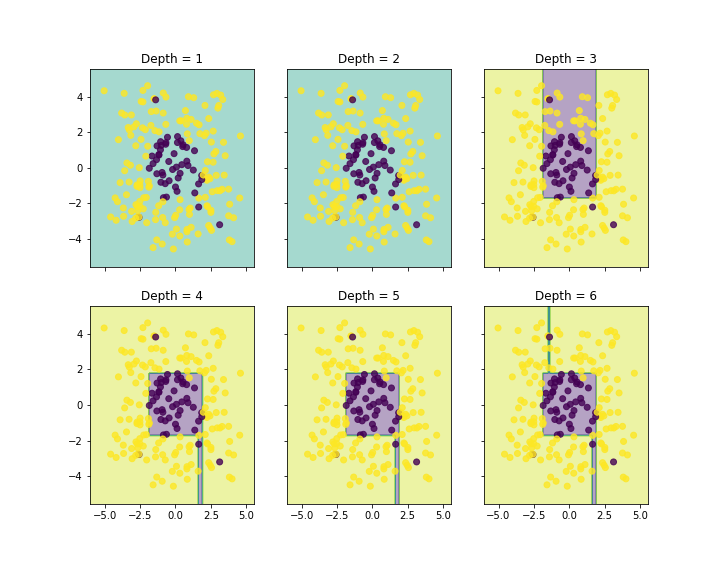
\includegraphics[width=\textwidth]{DT_entropy.png}
\end{figure}

\pagebreak
\text{  }
\\
\pagebreak
\item {[}Optional{]} Complete the function mean\_absolute\_deviation\_around\_median
(MAE). Use the code provided to fit the Regression\_Tree to the krr
dataset using both the MAE loss and median predictions. Include the
plots for the 6 fits.
%%%%%%%%%%%%%%%%%%%%%%%%%%%%%%%%%%%%%%%%%%%%%%%%%%%%%%%%%%%%%%%%
% 5.1Answer
%%%%%%%%%%%%%%%%%%%%%%%%%%%%%%%%%%%%%%%%%%%%%%%%%%%%%%%%%%%%%%%%
\\
\noindent\rule{14.3cm}{2pt}\\
\textbf{Answer:}\\
\textbf{The following are codes for MAE loss and the results of decision tree implemented on regression data}\\
\begin{minted}{python}
# Regression Tree Specific Code
def mean_absolute_deviation_around_median(y):
    '''
    Calulate the mean absolute deviation around the median of a given target list
    
    :param y: a numpy array of targets shape = (n, 1)
    :return mae
    '''
    # Your code goes here
    median = np.median(y)
    mae = np.mean(np.abs(y-median))
    return mae
\end{minted}
\begin{figure}
\caption{Decision Tree regression with MAE loss implemented}
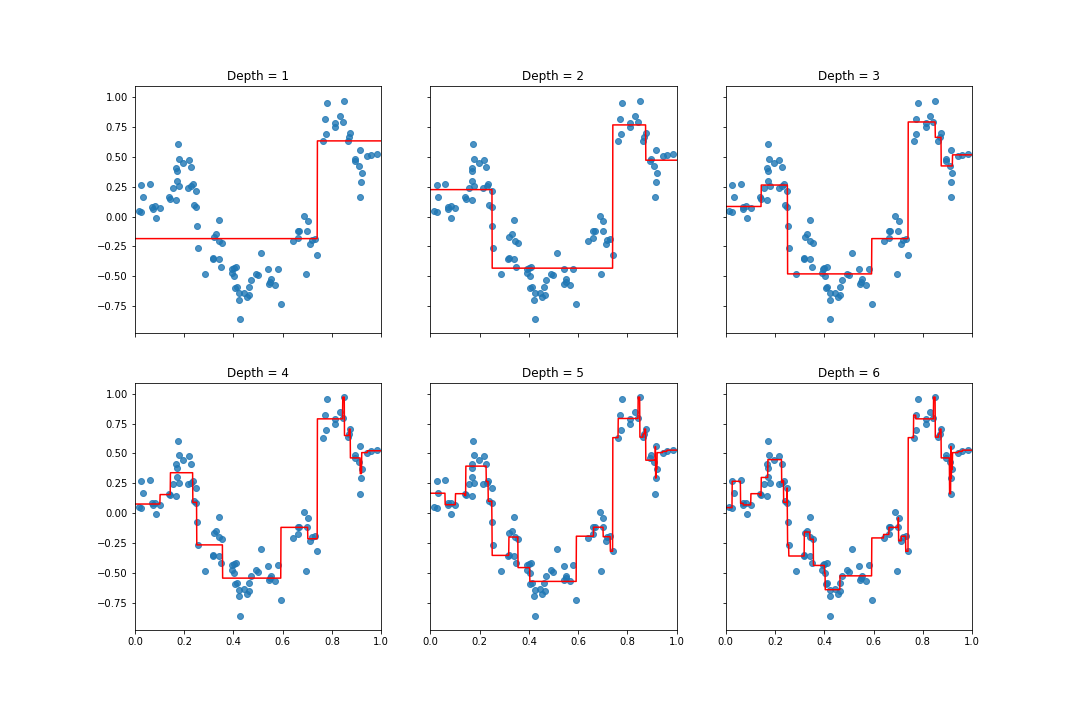
\includegraphics[width=\textwidth]{DT_regression.png}
\end{figure}
\end{enumerate}

\pagebreak
\section{Gradient Boosting Implementation}

This method goes by many names, including gradient boosting machines
(GBM), generalized boosting models (GBM), AnyBoost, and gradient boosted
regression trees (GBRT), among others. Although one of the nice aspects
of gradient boosting is that it can be applied to any problem with
a subdifferentiable loss function, here we'll keep things simple and
consider the standard regression setting with square loss. 
\begin{enumerate}
	\item Complete the gradient\_boosting class. As the base regression algorithm,
	you should use the regression tree from the previous problem, if you
	completed it. Otherwise, you may use sklearn's regression tree. You
	should use the square loss for the tree splitting rule and the mean
	function for the leaf prediction rule. Run the code provided to build
	gradient boosting models on the classification and regression data
	sets, and include the plots generated. Note that we are using square
	loss to fit the classification data, as well as the regression data.
\include{file}
%%%%%%%%%%%%%%%%%%%%%%%%%%%%%%%%%%%%%%%%%%%%%%%%%%%%%%%%%%%%%%%%
% 6.1 Answer
%%%%%%%%%%%%%%%%%%%%%%%%%%%%%%%%%%%%%%%%%%%%%%%%%%%%%%%%%%%%%%%%
\noindent\rule{14.3cm}{2pt}\\
\textbf{Answer:}\\
\text{Result:}
\begin{figure}[ht]
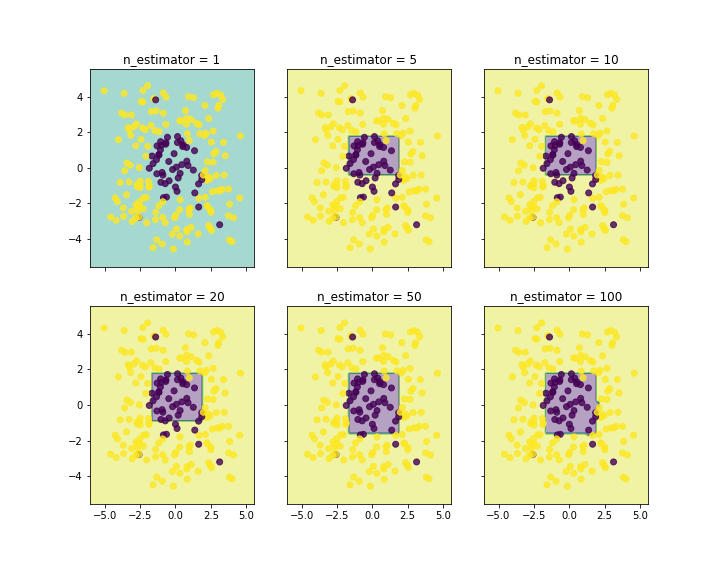
\includegraphics[width=\textwidth]{GBM_l2.png}
\caption{Gradient Boosting Tree with l2-loss}
\end{figure}

\begin{figure}[ht]
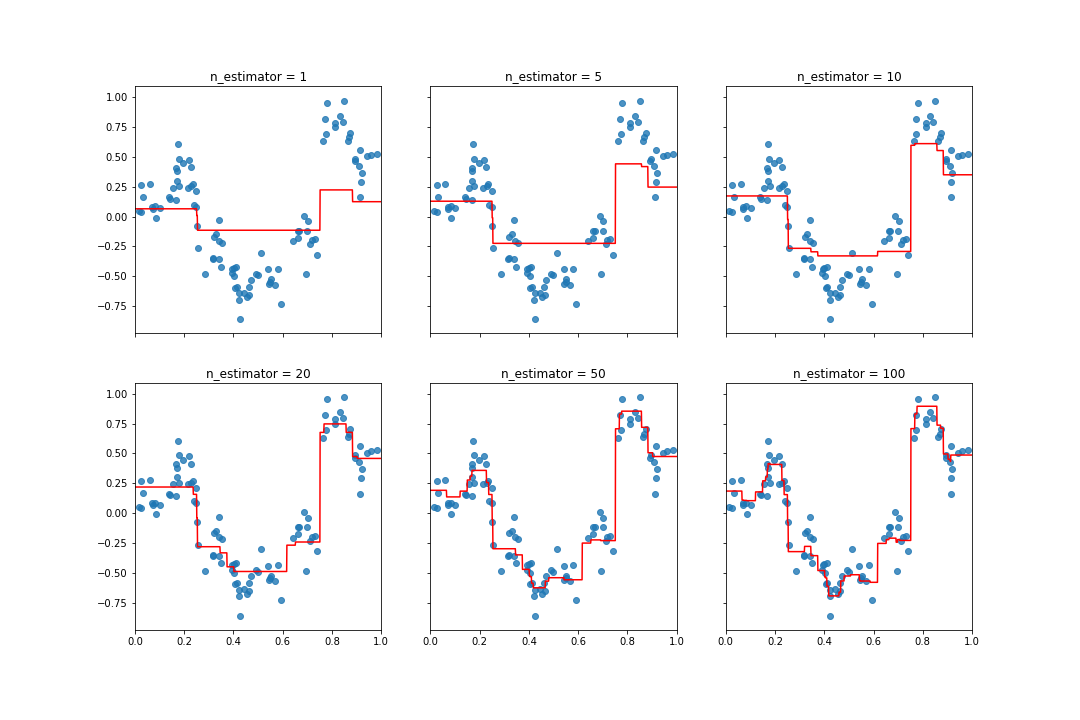
\includegraphics[width=\textwidth]{GBM_regression.png}
\caption{Gradient Boosting Regression}
\end{figure}
\textbf{Following is my result and code for GBM:}

\begin{minted}{python}
class gradient_boosting():
 '''
 Gradient Boosting regressor class
 :method fit: fitting model
 '''
 def __init__(self, n_estimator, pseudo_residual_func,\
              learning_rate=0.1, min_sample=5, max_depth=3):
     '''
     Initialize gradient boosting class
     
     :param n_estimator: number of estimators (i.e. number of rounds of gradient boosting)
     :pseudo_residual_func: function used for computing pseudo-residual
     :param learning_rate: step size of gradient descent
     '''
     self.n_estimator = n_estimator
     self.pseudo_residual_func = pseudo_residual_func
     self.learning_rate = learning_rate
     self.min_sample = min_sample
     self.max_depth = max_depth
     ##########
     #Note: Should be optimized so that the model does not waste memory
     #list for saving hm for each step and the 
     self.base_models = []
     self.f0 = None
     ##########
 def fit(self, train_data, train_target):
     '''
     Fit gradient boosting model
     '''
     #Fit base model f0 
     #Note: My f0 may looks like others h1 since I did not initialized f0=0 
     self.f0 = DecisionTreeRegressor(max_depth=self.max_depth,\
                                     min_samples_leaf=self.min_sample)
     self.f0.fit(train_data,train_target)
     for step in range(self.n_estimator):
         step_prediction = self.learning_rate*self.f0.predict(train_data)
         #If there is not model in list direcly calculate residuals with f0
         if len(self.base_models)==0:
             residuals = self.pseudo_residual_func(train_target.reshape(-1),\
                                                   step_prediction)
         else:
             for i in range(len(self.base_models)):
                 #Calculate prediction using weight sum of predictions of hm_s
                 step_prediction += \
                 self.learning_rate*self.base_models[i].predict(train_data)
             #Calculate residuals with fm(x)
             #Notice: sometimes y_train is of (-1,1) shape we need to reshape to (-1)
             residuals = self.pseudo_residual_func(train_target.reshape(-1)\
                                                   ,step_prediction)
         #Fit hm to residuals, which is some negative gradient direction
         hm = DecisionTreeRegressor(max_depth=self.max_depth,\
                                    min_samples_leaf=self.min_sample)
         hm.fit(train_data,residuals)
         #Update hm list
         self.base_models.append(hm)
     
 def predict(self, test_data):
     '''
     Predict value
     '''
     step_prediction = 0.2*self.f0.predict(test_data)
     for i in range(len(self.base_models)):
         #Get fm(x) by summation of base predictions
         step_prediction += self.learning_rate*\
         self.base_models[i].predict(test_data)
     return step_prediction
\end{minted}
	
	
	\pagebreak
	
	
	
	
	\item {[}Optional{]} Repeat the previous runs on the classification data
	set, but use a different classification loss, such as logistic loss
	or hinge loss. Include the new code and plots of your results. Note
	that you should still use the same regression tree settings for the
	base regression algorithm. 
	%%%%%%%%%%%%%%%%%%%%%%%%%%%%%%%%%%%%%%%%%%%%%%%%%%%%%%%%%%%%%%%%
	% 6.1 Answer
	%%%%%%%%%%%%%%%%%%%%%%%%%%%%%%%%%%%%%%%%%%%%%%%%%%%%%%%%%%%%%%%%
	\noindent\rule{14.3cm}{2pt}\\
	\textbf{Answer:}\\
	\text{Result:}\\
	\begin{figure}[ht]
	\caption{Gradient Boosting Tree with logistic lost}
	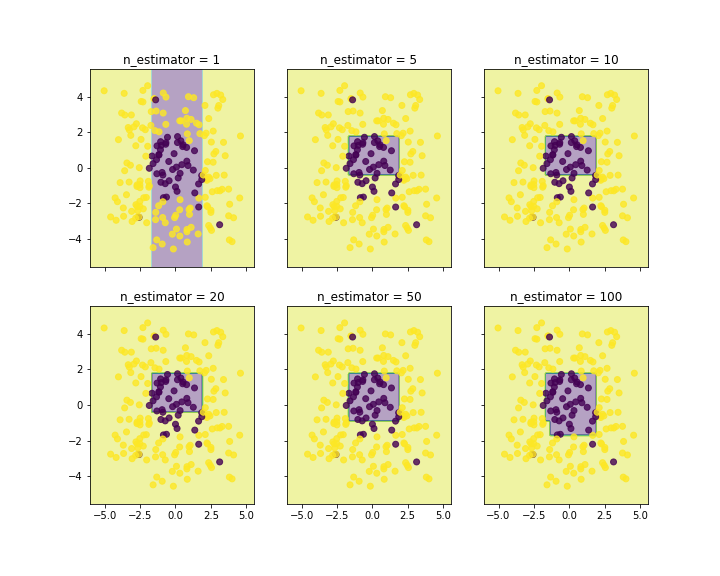
\includegraphics[width=\textwidth]{GBM_logistic.png}
	\end{figure}
	\begin{minted}{python}
	def pseudo_residual_logistic(train_target,train_predict):
	    y = train_target
	    fx = train_predict
	    m = y*fx
	    return (y*np.exp(-m))/(1+np.exp(-m))
	\end{minted}
\end{enumerate}



\end{document}


